\scanpage{106}
% archive foliation: 105
Montpellier \unsure{le|be} 11.1.1977

\deleted{Monsieur le Ministre,

Je me permets de recommander à votre attention le jeune mathéma-\newline
 ticien Kwang Taek Jeong, Chargé de Cours}

\figure{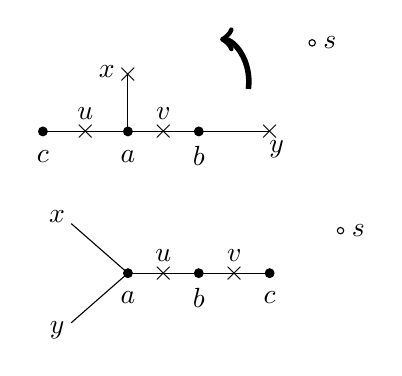
\begin{tikzpicture}[scale=.9]
\draw(-1.2,0)--(2,0);\draw(0,0)--(0,.8);\fill(-1.2,0)circle(.07);\fill(0,0)circle(.07);\fill(1,0)circle(.07);\node at(2,0){$\times$};\node at(0,.8){$\times$};\node at(-.6,0){$\times$};\node at(.5,0){$\times$};
\node at(-1.2,-.35){$c$};\node at(0,-.35){$a$};\node at(1,-.35){$b$};\node at(2.1,-.25){$y$};\node at(-.3,.85){$x$};\node at(-.6,.25){$u$};\node at(.5,.25){$v$};\draw(2.6,1.25)circle(.045);\node at(2.85,1.25){$s$};\draw[->,line width=2pt](1.7,.6)..controls(1.75,1)and(1.5,1.3)..(1.3,1.3);
\begin{scope}[yshift=-2cm]
\draw(-.8,.7)--(0,0)--(-.8,-.7);\draw(0,0)--(2,0);\fill(0,0)circle(.07);\fill(1,0)circle(.07);\fill(2,0)circle(.07);\node at(.5,0){$\times$};\node at(1.5,0){$\times$};\node at(-1,.8){$x$};\node at(-1,-.8){$y$};\node at(0,-.35){$a$};\node at(1,-.35){$b$};\node at(2,-.35){$c$};\node at(.5,.25){$u$};\node at(1.5,.25){$v$};\draw(3,.6)circle(.045);\node at(3.25,.6){$s$};\end{scope}
\end{tikzpicture}}
\diagram{$\begin{array}{ccc}3&2_2&\\2&1_2&6\\1&&\end{array}$}
\[\sigma_2\sigma_1\sigma_{\unsure1}\sigma_{\unsure2}=\]
\[\rho_s\rho_f=\sigma\qquad\rho_f=\rho_s^{-1}\sigma\]

\textcircled{I}
\diagram{$\begin{array}{llll}
r_1=(a,\unsure{ab})&\rho_s r_1=r_2&\sigma r_1=r_4&\rho_f r_1=r_5\\
r_2=(a,axa)&\rho_s r_2=r_3&\sigma r_4=r_1&\rho_f r_5=r_4\\
r_3=(a,ac)&\rho_s r_3=r_1&\sigma r_2=r_2&\rho_f r_4=r_3\\
r_4=(b,ba)&\rho_s r_4=r_5&\sigma r_3=r_6&\rho_f r_3=r_6\\
r_5=(b,byb)&\rho_s r_5=r_4&\sigma r_{\unsure6}=r_3&\rho_f r_6=r_2\\
r_6=(c,ca)&\rho_s r_6=r_6&\sigma r_5=r_5&\rho_f r_2=r_1
\end{array}$}
\figure{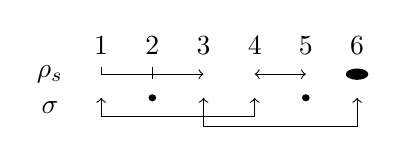
\begin{tikzpicture}[x=.65cm,y=.6cm]
\foreach\x in{1,...,6}{\node at(\x,1){$\x$};}
\node at(0,.4){$\rho_s$};\draw[->](1,.4)--(3,.4);\draw(1,.4)--(1,.55);\draw(2,.3)--(2,.55);\draw[<->](4,.4)--(5,.4);\fill(6,.4)ellipse(.22 and .12);
\node at(0,-.3){$\sigma$};\draw[<->](1,-.1)--(1,-.5)--(4,-.5)--(4,-.1);\draw[<->](3,-.1)--(3,-.7)--(6,-.7)--(6,-.1);\fill(2,-.1)circle(.075);\fill(5,-.1)circle(.075);
\end{tikzpicture}}
$\mathbb Z/6\mathbb Z$
\[p=6\quad q=2\quad r=6\]
\[N=\]

\textcircled{II}
\figure{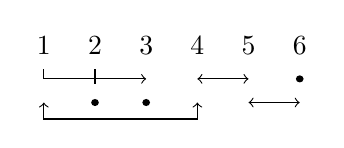
\begin{tikzpicture}[x=.65cm,y=.6cm]
\foreach\x in{1,...,6}{\node at(\x,1){$\x$};}
\draw[->](1,.3)--(3,.3);\draw(1,.3)--(1,.5);\draw(2,.2)--(2,.5);\draw[<->](4,.3)--(5,.3);\fill(6,.3)circle(.075);
\draw[<->](1,-.2)--(1,-.55)--(4,-.55)--(4,-.2);\fill(2,-.2)circle(.075);\fill(3,-.2)circle(.075);\draw[<->](5,-.2)--(6,-.2);
\end{tikzpicture}}
\diagram{$\begin{array}{llll}
r_1=(a,ab)&\rho_s r_1=r_2&\sigma r_1=r_4&\rho_f r_1=r_5\\
r_2=(a,axa)&\rho_s r_2=r_3&\sigma\unsure{\Delta}r_4=r_1&\rho_f r_5=r_6\\
r_3=(a,aya)&\rho_s r_3=r_1&\sigma r_2=r_2&\rho_f r_6=r_4\\
r_4=(b,ba)&\rho_s r_4=r_5&\sigma r_3=r_3&\rho_f r_4=r_3\\
r_5=(b,bc)&\rho_s r_5=r_{\unsure{4|2}}&\sigma r_5=r_6&\rho_f r_3=r_2\\
r_6=(c,cb)&\rho_s r_6=r_6&\sigma r_6=r_5&\rho_f r_2=r_1
\end{array}$}
